\documentclass[letterpaper,12pt,fleqn]{article}
\usepackage{matharticle}
\pagestyle{empty}

\renewcommand{\d}{\delta}
\newcommand{\e}{\epsilon}

\begin{document}

\section*{Arbitrarily Close}

\begin{itemize}[left=0in]
\item Everything that we can do in algebra is ultimately based on three things:
  \begin{enumerate}
  \item The substitution principle.
  \item The closed and well-defined nature of addition and multiplication.
  \item The nine real number (field) axioms.
  \end{enumerate}

\item But there are some problems that algebra cannot solve:
  \begin{enumerate}
  \item The slope of a tangent line to a non-linear curve.
  \item The area under a non-linear curve.
  \end{enumerate}

\item A new concept is needed to solve problems that algebra alone cannot solve: arbitrarily close.
\end{itemize}

\bigskip

\begin{center}
  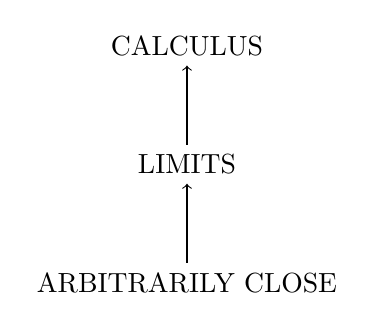
\begin{tikzpicture}
    \node (C) at (0,3) {CALCULUS};
    \node (L) at (0,1.5) {LIMITS};
    \node (A) at (0,0) {ARBITRARILY CLOSE};
    \draw [<-] (C) to (L);
    \draw [<-] (L) to (A);
  \end{tikzpicture}
\end{center}

\bigskip

\begin{center}
  \fbox{
    \begin{minipage}{6in}
      \bigskip

      Q: What is meant by saying that one thing is \emph{close} to another?
      
      \bigskip

      A: The \emph{distance} between them is \emph{small}.

      \bigskip
    \end{minipage}
  }
\end{center}  

\bigskip

But this is a subjective statement.  In math, we want objective facts.

\begin{definition}[Distance]
  Let \(a,b\in\R\).  The \emph{distance} from \(a\) to \(b\) is given by:
  \[d(a,b)=\abs{b-a}\]
\end{definition}

\bigskip

\begin{center}
  \begin{tikzpicture}
    \draw [fill,green] (-1,-0.25) rectangle (2,0.25);
    \draw [<->] (-3,0) -- (4,0);
    \node (a) [closed point] at (-1,0) {};
    \node [below,text height=1.5ex] at (a) {\(a\)};
    \node (b) [closed point] at (2,0) {};
    \node [below,text height=1.5ex] at (b) {\(b\)};
  \end{tikzpicture}
\end{center}

\begin{properties}[Distance]
  \begin{enumerate}
  \item[]
  \item \(d(a,b)=\abs{b-a}=\abs{a-b}=d(b,a)\)
  \item \(d(a,0)=\abs{a-0}=\abs{a}\)
  \end{enumerate}
\end{properties}

Let \(\e>0\).  By the density of \(\R\), there always exists some \(x\) such that \(0<x<\e\).

\bigskip

\begin{center}
  \begin{tikzpicture}
    \draw [<->] (0,0) -- (6,0);
    \node (z) [closed point] at (1,0) {};
    \node [below,text height=1.5ex] at (z) {\(0\)};
    \node (x) [closed point] at (3,0) {};
    \node [below,text height=1.5ex] at (x) {\(x\)};
    \node (e) [closed point] at (5,0) {};
    \node [below,text height=1.5ex] at (e) {\(\e\)};
  \end{tikzpicture}
\end{center}

\begin{example}
  Consider the following game:
  \begin{enumerate}
  \item Select some \(\e>0\).
  \item\label{step:select} Select some \(x\in(0,\e)\).
  \item Let \(\e=x\).
  \item Go to step \ref{step:select}.
  \end{enumerate}

  \[\begin{array}{l}
  1 \\
  \\
  \frac{1}{2} \\
  \\
  \frac{1}{4} \\
  \\
  \frac{1}{8} \\
  \\
  0.1 \\
  \\
  0.0001 \\
  \\
  0.00005 \\
  \\
  0.00000000001 \\
  \\
  \vdots
  \end{array}\]
\end{example}

\begin{definition}[Arbitrarily Small]
  To say that a value \(x\in\R\) is \emph{arbitrarily small} means that for every \(\e>0,0<x<\e\).
\end{definition}

\begin{itemize}[left=0in]
\item This does not imply that \(x\) is assigned a particular value nor does it say that \(x=0\).
\item It is indicative of an infinite argument: no matter which \(\e\) is selected, \(x\) is smaller (less) than
  \(\e\) (but not \(0\)).
\item It is tempting to think of \(\e\) constantly decreasing, pushing \(x\) continually closer to \(0\); however,
  this is imprecise: there are ways to continually decrease \(\e\) such that \(x\) gets no closer to \(0\).
\end{itemize}

\begin{example}
  Consider \(\e>2\) and \(x=1\).  Now, for each step, move \(\e\) to the halfway point between the previous
  \(\e\) and \(2\).  Although \(\e\) is continually getting smaller, \(x\) is not forced to move.

  \bigskip

  \begin{center}
    \begin{tikzpicture}
      \draw [<->] (-1,0) -- (5,0);
      \node (z) [closed point] at (0,0) {};
      \node [below,text height=1.5ex] at (z) {\(0\)};
      \node (o) [closed point] at (1,0) {};
      \node [below,text height=1.5ex] at (o) {\(x=1\)};
      \node (t) [closed point] at (2,0) {};
      \node [below,text height=1.5ex] at (t) {\(2\)};
      \node (e1) [closed point] at (4,0) {};
      \node [below,text height=1.5ex] at (e1) {\(\e_1\)};
      \node (e2) [closed point] at (3,0) {};
      \node [below,text height=1.5ex] at (e2) {\(\e_2\)};
    \end{tikzpicture}
  \end{center}

  The problem is that values of \(\e\le2\) are not considered.
\end{example}

\begin{definition}[Arbitrarily Close]
  To say that a value \(x\in\R\) is \emph{arbitrarily close} to another value \(a\in\R\), denoted by \(x\to a\),
  means that the distance between \(x\) and \(a\) becomes arbitrarily small (but not 0):
  \[\forall\,\e>0,0<\abs{x-a}<\e\]
\end{definition}

This means that for every \(\e>0\), \(a-\e<x<a+\e\):

\bigskip

\begin{center}
  \begin{tikzpicture}
    \draw [<->] (-4,0) -- (4,0);
    \node (a) [closed point] at (0,0) {};
    \node [below] at (a) {\(a\)};
    \node (ape) [closed point] at (2,0) {};
    \node [below] at (ape) {\(a+\e\)};
    \node (ame) [closed point] at (-2,0) {};
    \node [below] at (ame) {\(a-\e\)};
    \node (x) [closed point,red] at (1,0) {};
    \node [below] at (x) {\(x\)};

    \draw [<->] (-4,-2) -- (4,-2);
    \node (a) [closed point] at (0,-2) {};
    \node [below] at (a) {\(a\)};
    \node (ape) [closed point] at (2,-2) {};
    \node [below] at (ape) {\(a+\e\)};
    \node (ame) [closed point] at (-2,-2) {};
    \node [below] at (ame) {\(a-\e\)};
    \node (x) [closed point,red] at (-1,-2) {};
    \node [below] at (x) {\(x\)};
  \end{tikzpicture}
\end{center}

\begin{definition}[Neighborhood]
  Let \(x,\e\in\R\) such that \(\e>0\).  The open interval \((x-\e,x+\e)\) is called an \emph{\(\e\)-neighbohood}
  of \(x\).
\end{definition}

\begin{notation}[One-sided]
Note that \(x\to a\) implies that \(x\) can approach \(a\) from either direction (from the left or from the right).
When we are only interested in one direction:

\bigskip

\begin{center}
  \begin{tabular}{|c|l|}
    \hline
    \(x\to a^+\) & \(x\) approaches from the right of \(a\) \\
    \hline
    \(x\to a^-\) & \(x\) approaches from the left of \(a\) \\
    \hline
  \end{tabular}
\end{center}

\bigskip

If the direction is understood then the direction indicator can be omitted.  For example, if \(x>0\) then
\(x\to0^+\) can be written as just \(x\to0\), which can be used to represent the fact that \(x\) gets arbitrarily
small.
\end{notation}

\newpage

\begin{example}
  Recall that one of the ways of representing a rational number is a terminating infinite repeating sequence of
  decimal digits.  For example:
  \[\frac{1}{9}=0.11111\ldots=0.\overline{1}\]
  It is easy to mark \(\frac{1}{9}\) on the number line.  But how does \(0.\overline{1}\) correspond to this point?
  As each repeated digit is added, the value \(0.\overline{1}\) gets \emph{arbitrarily close} to \(\frac{1}{9}\).
  For every \(\e>0\), enough digits can be added so that the result is eventually within \(\e\) of \(\frac{1}{9}\).

  \bigskip

  \begin{center}
    \begin{tikzpicture}
      \draw [<->] (-1,0) -- (4,0);
      \node (x) [closed point] at (0,0) {};
      \node [below] at (x) {\(0\)};
      \node (y) [closed point] at (3,0) {};
      \node [below] at (y) {\(\frac{1}{9}\)};
      \node (z) at (2,0) {\((\)};
      \node [below] at (z) {\(\frac{1}{9}-\e\)};
      \node (z) [closed point,red] at (2.5,0) {};
    \end{tikzpicture}
  \end{center}

  How many digits are required for \(\e=0.001\)?
  \[0.\bar{9}-0.9=0.0\bar{9}>0.001\]
  \[0.\bar{9}-0.99=0.00\bar{9}>0.001\]
  \[0.\bar{9}-0.999=0.000\bar{9}=0.001\]
  \[0.\bar{9}-0.9999=0.0000\bar{9}=0.0001<0.001\]
\end{example}

\begin{example}
  This works for irrational numbers as well, which are represented by terminating infinite sequences of
  non-repeating digits.  Consider \(\pi=3.1415926\ldots\).  For every \(\e>0\), enough digits can be added so that
  the result is eventually within \(\e\) or \(\pi\).

  \bigskip

  \begin{center}
    \begin{tikzpicture}
      \draw [<->] (-1,0) -- (4,0);
      \node (x) [closed point] at (0,0) {};
      \node [below] at (x) {\(0\)};
      \node (y) [closed point] at (3,0) {};
      \node [below] at (y) {\(\pi\)};
      \node (z) at (2,0) {\((\)};
      \node [below] at (z) {\(\pi-\e\)};
      \node (z) [closed point,red] at (2.5,0) {};
    \end{tikzpicture}
  \end{center}

  How many digits are required for \(\e=0.001\)?
  \[3.1415926\ldots-3=0.1415926\ldots>0.001\]
  \[3.1415926\ldots-3.1=0.0415926\ldots>0.001\]
  \[3.1415926\ldots-3.14=0.0015926\ldots>0.001\]
  \[3.1415926\ldots-3.141=0.0005926\ldots<0.001\]
\end{example}

\newpage

\begin{example}
  Consider the real numbers \(\frac{1}{7}\), \(\pi\), and \(\e\).  How many digits in the decimal forms are required
  such that each value is within \(0.005\) and then \(0.000001\) of its corresponding exact value?
  \begin{align*}
    \frac{1}{7} &= 0.14285714\ldots \\
    \pi &= 3.14159265\ldots \\
    e &= 2.71828182\ldots
  \end{align*}
  \[\begin{array}{|c||c|c|c|}
  \hline
  & & & \\
  \e & \frac{1}{7} & \pi & e \\
  & & & \\
  \hline
  \hline
  0.0005 & 0.1428 & 3.1415 & 2.718 \\
  \hline
  0.000001 & 0.142857 & 3.141592 & 2.718281 \\
  \hline
  \end{array}\]
\end{example}

\bigskip

Also important is the negation:

\begin{definition}[Not Arbitrarily Close]
  To say that a value \(x\in\R\) is \emph{not arbitrarily close} to another value \(a\in\R\), denoted by
  \(x\not\to a\), means that means that there exists an \(\e>0\) such that \(\abs{x-a}\ge\e\).
\end{definition}

\bigskip

\begin{center}
  \begin{tikzpicture}
    \draw [<->] (-4,0) -- (4,0);
    \node (a) [closed point] at (0,0) {};
    \node [below] at (a) {\(a\)};
    \node (ape) [closed point] at (2,0) {};
    \node [below] at (ape) {\(a+\e\)};
    \node (ame) [closed point] at (-2,0) {};
    \node [below] at (ame) {\(a-\e\)};
    \node (x) [closed point,red] at (3,0) {};
    \node [below] at (x) {\(x\)};

    \draw [<->] (-4,-2) -- (4,-2);
    \node (a) [closed point] at (0,-2) {};
    \node [below] at (a) {\(a\)};
    \node (ape) [closed point] at (2,-2) {};
    \node [below] at (ape) {\(a+\e\)};
    \node (ame) [closed point] at (-2,-2) {};
    \node [below] at (ame) {\(a-\e\)};
    \node (x) [closed point,red] at (-3,-2) {};
    \node [below] at (x) {\(x\)};
  \end{tikzpicture}
\end{center}

Thus, there is always some finite gap between \(x\) and \(a\).

\begin{example}
  Why isn't \(24.57\bar{9}\) arbitrarily close to \(24.6\)?

  Since \(24.57\bar{9}\le24.58\):
  \[24.6-24.57\bar{9}\ge24.6-24.58=0.02\]
  So there exists \(\e=0.02\) such that \(24.6-24.57\bar{9}\ge\e\).
\end{example}

\end{document}
